\documentclass[12pt,a4paper]{article}
\usepackage[utf8]{inputenc}
\usepackage[T1]{fontenc}
\usepackage[brazil]{babel}
\usepackage{amsmath,amssymb}
\usepackage{booktabs}
\usepackage{float}
\usepackage{graphicx}
\usepackage[margin=2.5cm]{geometry}

\begin{document}

\setcounter{section}{1}
\setcounter{subsection}{4}

\subsection{Estimação por Máxima Verossimilhança (Itens 1.5c e 1.5d)}

Dando continuidade ao estudo da variável aleatória discreta que modela o número de requisições com processamento adicional em um serviço web, esta etapa tem como objetivo simular, na linguagem R, uma amostra finita de $n = 50$ requisições independentes e identicamente distribuídas (i.i.d.) com distribuição $\operatorname{Bernoulli}(p)$, utilizando a probabilidade teórica atribuída à equipe ($p = 0{,}08$, obtida a partir da maior matrícula $M = 581706$). Em seguida, calcula-se a estimativa de máxima verossimilhança (MLE) $\hat{p}$ e analisa-se o comportamento desse estimador em amostras finitas e sob o aumento do tamanho amostral. Toda a implementação computacional foi realizada utilizando apenas funções nativas do R (\texttt{rbinom()}, \texttt{mean()} e \texttt{plot()}), com semente aleatória fixada por meio de \texttt{set.seed(581706)} para garantir reprodutibilidade.

\subsubsection{Item 1.5(c): Simulação de Amostra Bernoulli e Cálculo do MLE}

Considerando uma amostra aleatória $X_1, X_2, \dots, X_n \stackrel{\text{i.i.d.}}{\sim} \operatorname{Bernoulli}(p)$, em que $X_i = 1$ indica uma requisição que exige processamento adicional e $X_i = 0$ indica uma requisição normal, o estimador de máxima verossimilhança derivado nos itens anteriores é dado pela proporção amostral de sucessos:
\[
\hat{p} = \frac{k}{n} = \bar{X}, \qquad k = \sum_{i=1}^{n} X_i.
\]

Para a simulação computacional, geraram-se $n = 50$ observações independentes de $\operatorname{Bernoulli}(0{,}08)$ em R por meio de \texttt{rbinom(50, size = 1, prob = 0.08)}, com semente fixada em \texttt{581706}. Na amostra gerada, observaram-se $k = 5$ requisições que exigiram processamento adicional, resultando na seguinte estimativa de máxima verossimilhança:
\[
\hat{p} = \frac{5}{50} = \mathbf{0{,}10}.
\]

\subsubsection{Item 1.5(d): Comparação com $p$ Teórico e Efeito do Tamanho Amostral}

Comparando a estimativa obtida ($\hat{p} = 0{,}10$) com a probabilidade teórica da equipe ($p = 0{,}08$), observa-se uma diferença absoluta de $|\hat{p} - p| = 0{,}02$, o que corresponde a um erro relativo de $25\%$ em relação ao valor teórico.

Essa divergência em uma amostra finita decorre de dois fatores principais:
\begin{enumerate}
    \item \textbf{Variabilidade amostral:} embora o valor esperado de sucessos em $50$ requisições seja $E[X] = np = 50 \cdot 0{,}08 = 4$, o processo aleatório pode produzir realizações ligeiramente acima ou abaixo da média; na amostra simulada, obteve-se $k = 5$. Como o erro padrão teórico do estimador para $n = 50$ é $EP(\hat{p}) = \sqrt{\frac{p(1-p)}{n}} = \sqrt{\frac{0{,}08 \cdot 0{,}92}{50}} \approx 0{,}0384$, a diferença observada de $0{,}02$ situa-se dentro da faixa esperada de flutuação amostral (menor que um erro padrão).
    \item \textbf{Discretização do estimador:} como $k$ assume apenas valores inteiros, a estimativa $\hat{p} = k/50$ só pode variar em incrementos múltiplos de $1/50 = 0{,}02$. Assim, o desvio de apenas uma requisição em relação ao valor esperado já desloca $\hat{p}$ em $0{,}02$.
\end{enumerate}

Para avaliar o efeito do tamanho amostral $n$ sobre a estimação, geraram-se amostras adicionais com $n \in \{50, 500, 5000, 50000\}$ mantendo $p = 0{,}08$. Os resultados estão resumidos na Tabela~\ref{tab:mle_tamanhos} e ilustrados na Figura~\ref{fig:mle_convergencia}.

\begin{table}[H]
\centering
\caption{Estimativas de máxima verossimilhança $\hat{p}$ e erro absoluto para diferentes tamanhos amostrais ($p = 0{,}08$).}
\label{tab:mle_tamanhos}
\begin{tabular}{@{}lcc@{}}
\toprule
\textbf{Tamanho da amostra ($n$)} & \textbf{Estimativa ($\hat{p}$)} & \textbf{Erro absoluto ($|\hat{p} - p|$)} \\ \midrule
$50$     & $0{,}10000$ & $0{,}02000$ \\
$500$    & $0{,}07200$ & $0{,}00800$ \\
$5000$   & $0{,}07400$ & $0{,}00600$ \\
$50000$  & $0{,}08076$ & $0{,}00076$ \\ \bottomrule
\end{tabular}
\end{table}

\begin{figure}[H]
\centering
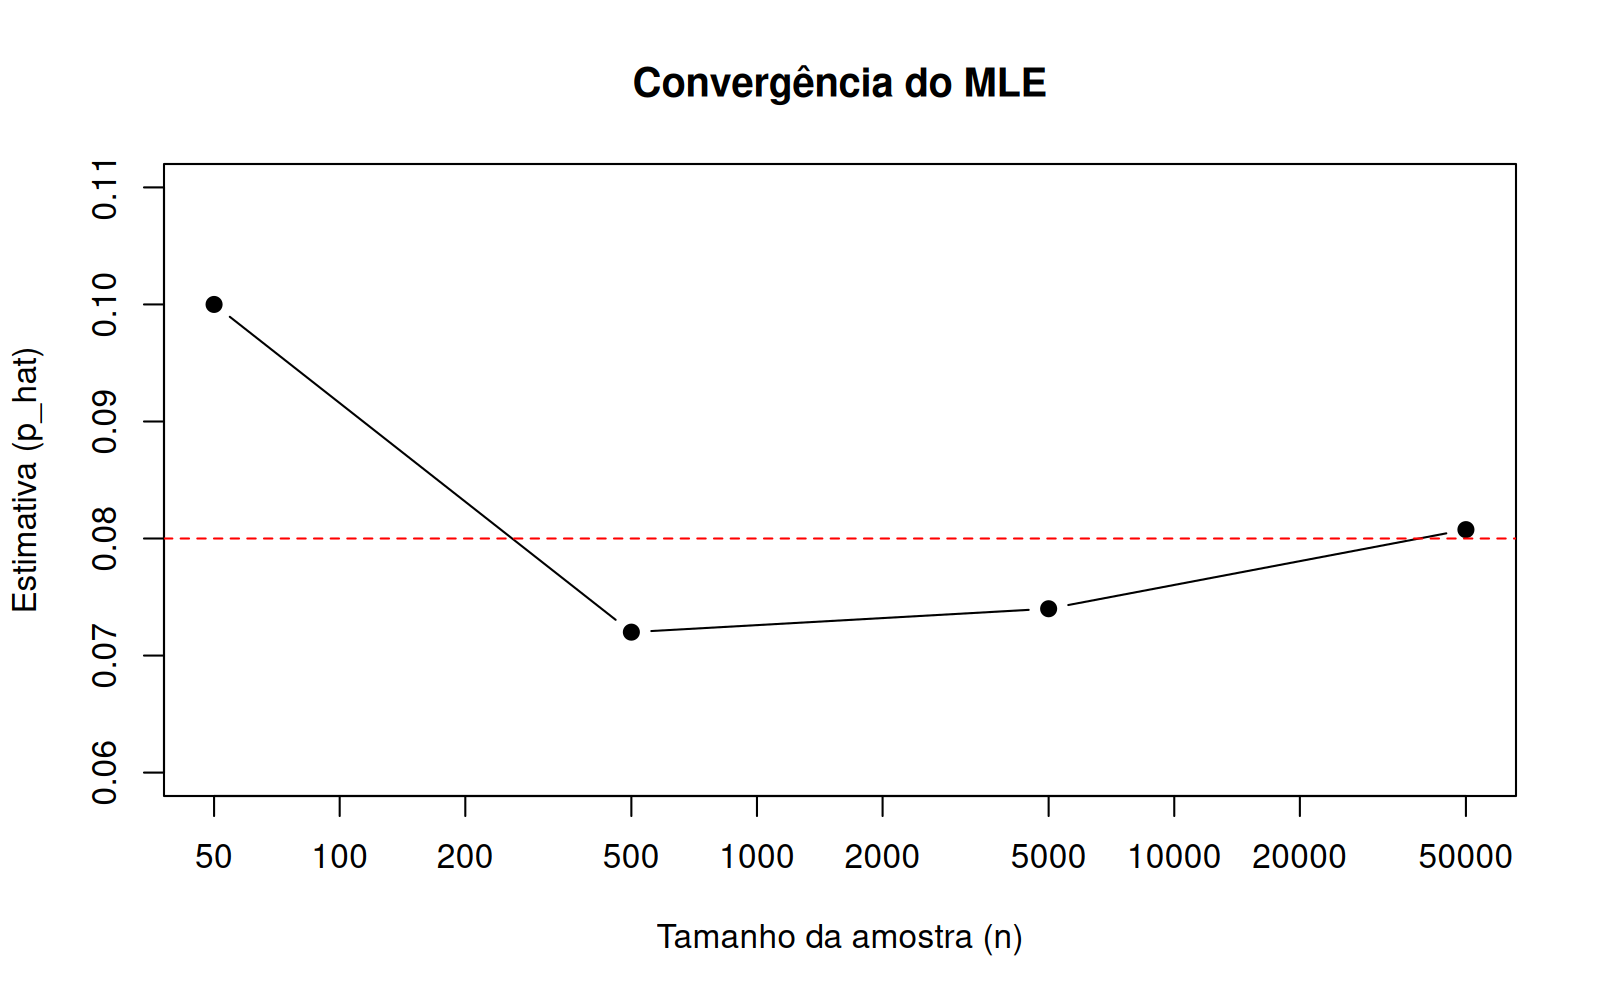
\includegraphics[width=0.75\textwidth]{../imagens/mle_convergencia.png}
\caption{Convergência da estimativa de máxima verossimilhança $\hat{p}$ para o parâmetro teórico $p = 0{,}08$ conforme o aumento do tamanho amostral $n$.}
\label{fig:mle_convergencia}
\end{figure}

Observa-se que, à medida que $n$ cresce, o erro absoluto reduz-se expressivamente, passando de $0{,}02000$ em $n = 50$ para $0{,}00076$ em $n = 50000$. Esse comportamento é explicado pela variância do estimador, $\operatorname{Var}(\hat{p}) = \frac{p(1-p)}{n}$, que decresce inversamente com $n$ (fazendo o erro padrão diminuir na razão de $1/\sqrt{n}$), bem como pela redução do passo mínimo $1/n$ entre estimativas possíveis. Pela Lei dos Grandes Números, $\hat{p}$ converge em probabilidade para o parâmetro verdadeiro $p$ quando $n \to \infty$, evidenciando a consistência do estimador de máxima verossimilhança.

\end{document}
